\documentclass[letterpaper,twocolumn,10pt]{article}
\usepackage{usenix-2019-v3}
\usepackage{booktabs}

% to be able to draw some self-contained figs
\usepackage{tikz}
% inlined bib file
\usepackage{filecontents}
\usepackage{bm}       % 若后续需要粗体数学符号（可选）
\usepackage{amsmath, amssymb, amsfonts}
\usepackage{graphicx}
\usepackage{algorithm}
\usepackage{algpseudocode}
\usepackage{booktabs}
\usepackage{multirow}
\usepackage{color}



\begin{document}
%-------------------------------------------------------------------------------

%don't want date printed
\date{}

% make title bold and 14 pt font (Latex default is non-bold, 16 pt)
\title{\Large \bf GLaSS: Global Load-aware Scheduling for Spiking Neural Networks}

%for single author (just remove % characters)
\author{
{\rm Your N.\ Here}\\
Your Institution
\and
{\rm Second Name}\\
Second Institution
% copy the following lines to add more authors
% \and
% {\rm Name}\\
%Name Institution
} % end author

\maketitle

%-------------------------------------------------------------------------------
\begin{abstract}
~\cite{288610}Neuromorphic computing offers a promising energy-efficient paradigm for serving Spiking Neural Networks (SNNs). However, deploying SNNs as a cloud service faces significant challenges due to the unique spatio-temporal sparsity and bursty nature of spiking workloads. Traditional static scheduling policies (e.g., Best-Fit, DRF) fail to adapt to runtime workload fluctuations, leading to hardware hotspots and Service Level Agreement (SLA) violations. In this paper, we propose GLaSS, a Global Load-aware SNN Scheduler designed for multi-tenant neuromorphic clusters. GLaSS introduces a two-tier timing architecture that decouples physical execution from global scheduling to handle the high-frequency dynamics of SNNs. We propose a weighted spike-activity load metric and an ROI-Greedy migration strategy that dynamically rebalances workloads based on migration cost-efficiency. Extensive experiments demonstrate that GLaSS reduces load variance by over 70\% compared to static baselines and significantly improves system throughput under bursty traffic conditions.
\end{abstract}

\section{Introduction}
As Artificial Intelligence (AI) permeates web services, the energy consumption of deep learning models has become a bottleneck. Spiking Neural Networks (SNNs), running on neuromorphic hardware (e.g., Darwin3, Loihi), offer a sustainable alternative by leveraging event-driven computation. We envision a future of \textit{Neuromorphic Computing-as-a-Service} (NCaaS), where heterogeneous SNN tasks---from robotic control to sequential recommendation---share a unified hardware cluster.

However, serving SNNs in a multi-tenant environment presents unique challenges distinct from traditional DNN serving:
\begin{enumerate}
    \item \textbf{Stochastic Burstiness:} Unlike the deterministic compute graph of DNNs, SNN workloads are highly data-dependent. A "quiet" model may suddenly generate a spike burst, causing instantaneous congestion in the Network-on-Chip (NoC).
    \item \textbf{Static Binding Inflexibility:} Existing neuromorphic compilers typically employ static mapping strategies (e.g., Best-Fit or Dominant Resource Fairness). Once deployed, tasks are pinned to cores. When multiple co-located tasks burst simultaneously, "Head-of-Line" blocking occurs, degrading tail latency.
\end{enumerate}

To address these issues, we propose \textbf{GLaSS (Global Load-aware SNN Scheduler)}. Unlike general-purpose cluster schedulers (e.g., Kubernetes), GLaSS is aware of the neuro-synaptic dynamics.

Our key contributions are:
\begin{itemize}
    \item We propose a \textbf{Two-Tier Timing Architecture} that bridges the gap between millisecond-level physical execution and second-level global scheduling.
    \item We design a \textbf{Accumulated Spike-Activity Load} metric to accurately quantify the computational and communication pressure of SNNs.
    \item We develop an \textbf{ROI-Greedy Migration Strategy} that optimizes the trade-off between load balancing benefits and state migration costs ($S_{state}$).
    \item Evaluation shows GLaSS outperforms static baselines, reducing load imbalance by 73\% under bursty arrival patterns.
\end{itemize}
%-------------------------------------------------------------------------------
\section{Footnotes, Verbatim, and Citations}
%-------------------------------------------------------------------------------

Footnotes should be places after punctuation characters, without any
spaces between said characters and footnotes, like so.%
\footnote{Remember that USENIX format stopped using endnotes and is
  now using regular footnotes.} And some embedded literal code may
look as follows.

\begin{verbatim}
int main(int argc, char *argv[]) 
{
    return 0;
}
\end{verbatim}

Now we're going to cite somebody. Watch for the cite tag. Here it
comes. Arpachi-Dusseau and Arpachi-Dusseau co-authored an excellent OS
book, which is also really funny~\cite{arpachiDusseau18:osbook}, and
Waldspurger got into the SIGOPS hall-of-fame due to his seminal paper
about resource management in the ESX hypervisor~\cite{waldspurger02}.

The tilde character (\~{}) in the tex source means a non-breaking
space. This way, your reference will always be attached to the word
that preceded it, instead of going to the next line.

And the 'cite' package sorts your citations by their numerical order
of the corresponding references at the end of the paper, ridding you
from the need to notice that, e.g, ``Waldspurger'' appears after
``Arpachi-Dusseau'' when sorting references
alphabetically~\cite{waldspurger02,arpachiDusseau18:osbook}. 

It'd be nice and thoughtful of you to include a suitable link in each
and every bibtex entry that you use in your submission, to allow
reviewers (and other readers) to easily get to the cited work, as is
done in all entries found in the References section of this document.

Now we're going take a look at Section~\ref{sec:figs}, but not before
observing that refs to sections and citations and such are colored and
clickable in the PDF because of the packages we've included.

\section{Related Work}

\subsection{Maintaining the Integrity of the Specifications}

The IEEEtran class file is used to format your paper and style the text. All margins, 
column widths, line spaces, and text fonts are prescribed; please do not 
alter them. You may note peculiarities. For example, the head margin
measures proportionately more than is customary. This measurement 
and others are deliberate, using specifications that anticipate your paper 
as one part of the entire proceedings, and not as an independent document. 
Please do not revise any of the current designations.

\section{Preliminaries}
\subsection{SNN Service Model}
We consider a stream of SNN inference tasks submitted to the cluster. Each task $i$ is characterized by its neuron count $N_i$, synaptic weight storage $M_i$, and a time-varying firing rate $\lambda_i(t)$. The state size $S_{state}$ represents the context (membrane potentials, synaptic weights) that must be transferred during migration.

\subsection{Neuromorphic Cluster Resource}
The cluster consists of $M$ neuromorphic cards (nodes). Each card provides limited resources: Cores ($C$), Synaptic Memory ($S_{mem}$), and Routing Bandwidth ($B$).

\subsection{The Scheduling Problem}
The objective is to find a mapping function $\mathcal{M}: \text{Tasks} \to \text{Cards}$ that evolves over time to minimize the load variance across all cards, thereby minimizing queuing delay and maximizing cluster throughput.


\section{SYSTEM DESIGN}
The fundamental challenge in scheduling Spiking Neural Networks (SNNs) on a multi-card Compute-in-Memory (CIM) cluster (e.g., Darwin) lies in the \textit{Spatio-Temporal Coupling Calamity}. Unlike ANNs where execution flows are static and data-independent, SNNs generate discrete, highly time-varying, and input-dependent event streams (spikes). Traditional static scheduling formulates this as a Time-dependent Mixed-Integer Non-Linear Programming (MINLP) problem, which is inherently NP-Hard and suffers from state explosion, failing to prevent instantaneous Network-on-Chip (NoC) congestion. 

To break this bottleneck, we propose a two-stage Spatio-Temporal Proactive Scheduling (STPS) framework. It shifts the paradigm from \textit{reactive congestion handling} to \textit{proactive traffic shaping}. 

\subsection{System Architecture Overview}
Our framework decouples the MINLP problem into an offline workload profiling stage and an online hierarchical scheduling stage. 
\begin{itemize}
    \item \textbf{Offline Profiler:} Transforms the opaque, input-dependent SNN into a Discrete-Time Dynamic Graph (DTDG), extracting domain-invariant spatio-temporal fingerprints (e.g., burstiness, centrality).
    \item \textbf{Online STPS Scheduler:} Utilizes the extracted fingerprints to perform macro-level multi-card dispatching, micro-level spatial mapping, and most importantly, micro-level temporal phase-shifting to avoid NoC collision.
\end{itemize}

\begin{figure*}[t]
    \centering
    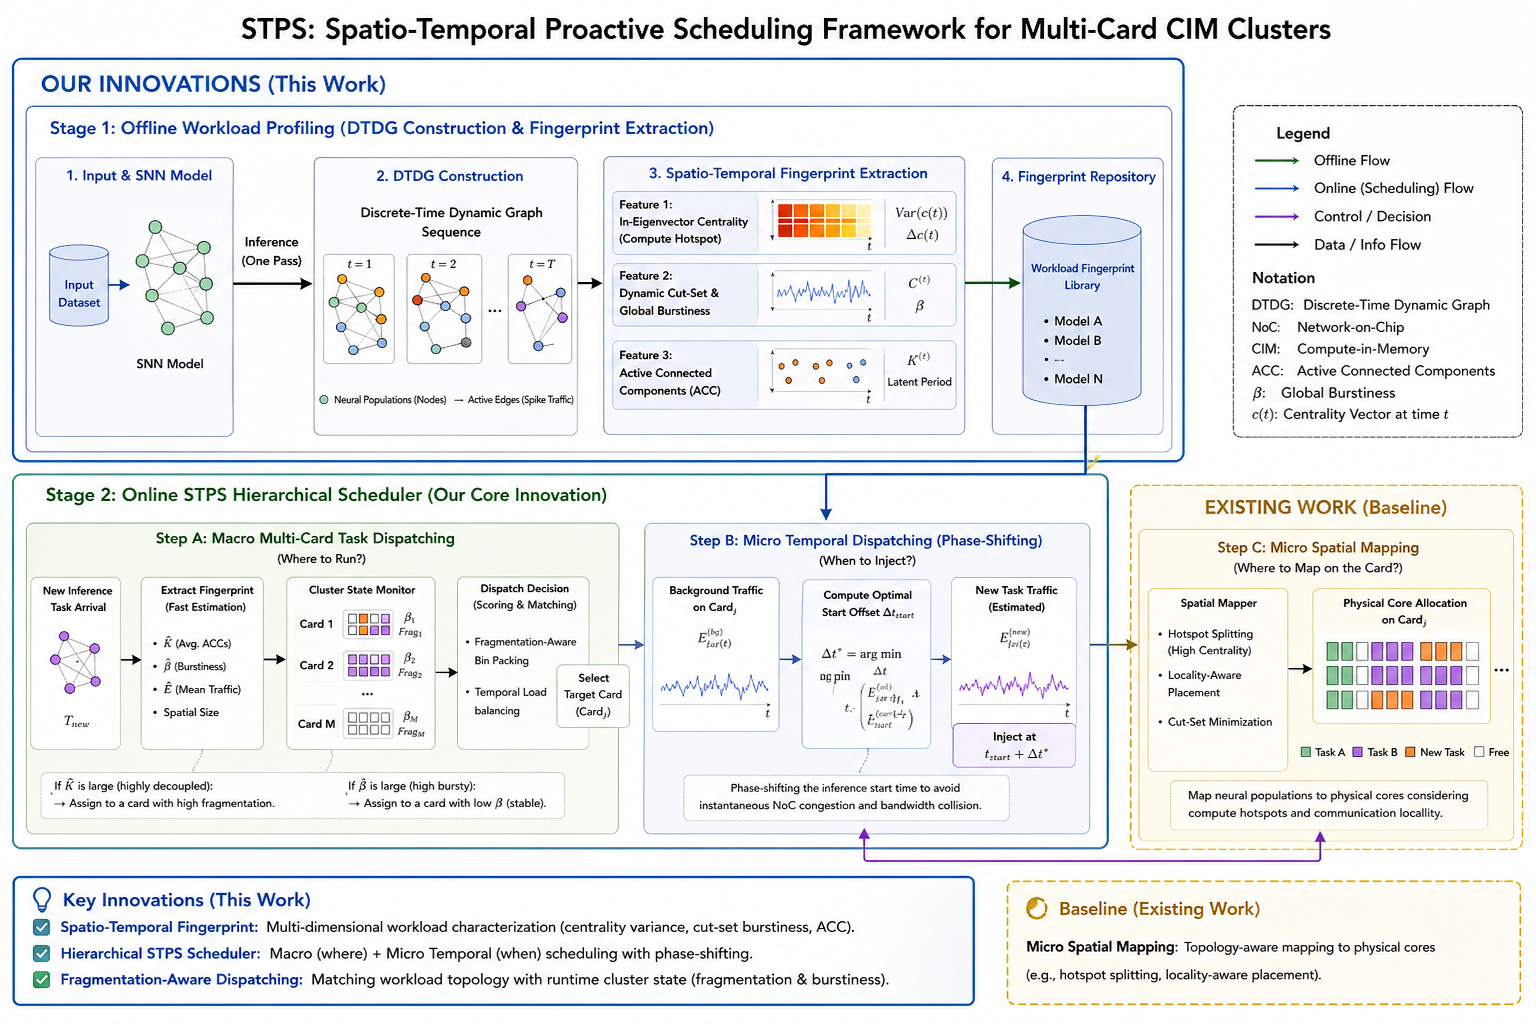
\includegraphics[width=\linewidth]{SNN schedule/picture/architecture.png}
    \caption{The proposed STPS framework for multi-card CIM clusters.}
    \label{fig:arch}
\end{figure*}

\subsection{Offline DTDG Workload Fingerprinting}
To eliminate the randomness caused by individual inputs, we feed a test dataset into the SNN simulator to extract the \textit{statistical expectation} of the spike traffic. The SNN workload is modeled as a DTDG sequence $\mathcal{G}_{dynamic} = \{ G^{(1)}, \dots, G^{(T_{window})} \}$.

At time step $t$, the dynamic graph $G^{(t)} = (\mathcal{V}, \mathcal{E}^{(t)}, \mathbf{W}^{(t)})$ models the neural populations $\mathcal{V}$ and their active event flows. The dynamic edge weight $w_{ij}^{(t)}$ from population $i$ to $j$ is decoupled into a 2D vector: NoC Traffic Volume and Compute Trigger (SOPs). 

Based on $G^{(t)}$, we extract three critical physical fingerprints to guide the system scheduling:
\begin{enumerate}
    \item \textbf{In-Eigenvector Centrality ($Var(\mathbf{c}^{(t)})$):} Measures the variance of compute hotspots. A high variance indicates severe local PIM array pressure. We use Power Iteration for $O(|\mathcal{E}^{(t)}|)$ fast approximation.
    \item \textbf{Global Burstiness ($\beta$) \& Traffic Sequence ($E^{(t)}$):} Defined as $\beta = \max_t (E^{(t)})/\mathbb{E}[E^{(t)}]$. It quantifies the tidal nature of the NoC traffic. $E^{(t)}$ is recorded as a 1D timeline vector for phase-shifting.
    \item \textbf{Active Connected Components ($\overline{K}$):} Represents the average number of decoupled sub-graphs. A high $\overline{K}$ indicates the model is highly fragmented and asynchronous.
\end{enumerate}

\subsection{Online Spatio-Temporal Proactive Scheduler}
When a new SNN inference task $T_{new}$ arrives, the online scheduler reads its DTDG fingerprint and executes a 3-stage hierarchical pipeline.

\subsubsection{Stage 1: Macro-Card Dispatching}
We solve the cross-card isolation constraint by formulating it as a fragmentation-aware and temporal-load-aware bin packing problem.
\begin{itemize}
    \item \textbf{Fragmentation Matching:} If $T_{new}$ is highly cohesive ($\overline{K} \to 1$), we allocate it to the card with the largest contiguous idle PIM cores. Conversely, if $T_{new}$ is highly decoupled (large $\overline{K}$), we assign it to heavily fragmented cards to maximize cluster utilization.
    \item \textbf{Temporal Load Isolation:} To avoid simultaneous NoC breakdowns across the cluster, we maintain a running average burstiness $\beta_{card}$ for each card. High-$\beta$ tasks are strictly dispatched to the card with the lowest $\beta_{card}$ (i.e., cards running smooth/flat tasks).
\end{itemize}

\subsubsection{Stage 2: Micro-Temporal Phase-Shifting}
\label{sec:phase_shift}
Once assigned to a target card $C_m$, the exact injection time of the input data dictates the runtime NoC congestion. Instead of letting tasks run blindly, we employ a sliding-window cross-correlation algorithm to find the optimal clock offset $\Delta t_{start}$.

Let $E_{m}^{(t)}$ be the forecasted background traffic timeline of card $C_m$, and $E_{new}^{(t)}$ be the fingerprint of the incoming task. The optimal offset minimizes the absolute peak traffic:
\begin{equation}
    \Delta t_{start}^* = \arg\min_{\Delta t \in [0, D_{max}]} \max_{t} \left( E_{m}^{(t)} + E_{new}^{(t - \Delta t)} \right)
\end{equation}
where $D_{max}$ is the maximum tolerable QoS delay. This transforms a 3D scheduling problem into a 1D convolution operation, executing in microseconds. 

\begin{algorithm}[h]
\caption{Temporal Phase-Shifting Dispatch}
\label{alg:phase_shift}
\begin{algorithmic}[1]
\State \textbf{Input:} Background traffic $E_{m}$, Task traffic $E_{new}$, Max delay $D_{max}$, Bandwidth $BW_{max}$
\State \textbf{Output:} Optimal offset $\Delta t_{start}^*$
\State $MinPeak \gets \infty$, $\Delta t_{start}^* \gets -1$
\For{$\Delta t = 0$ to $D_{max}$}
    \State $CombinedTraffic \gets E_{m} + \text{Shift}(E_{new}, \Delta t)$
    \State $CurrentPeak \gets \max(CombinedTraffic)$
    \If{$CurrentPeak \le BW_{max}$ \textbf{and} $CurrentPeak < MinPeak$}
        \State $MinPeak \gets CurrentPeak$
        \State $\Delta t_{start}^* \gets \Delta t$
    \EndIf
\EndFor
\State Update card state: $E_{m} \gets E_{m} + \text{Shift}(E_{new}, \Delta t_{start}^*)$
\State \textbf{return} $\Delta t_{start}^*$
\end{algorithmic}
\end{algorithm}

\subsubsection{Stage 3: Micro-Spatial Mapping}
Using the default practices of the Darwin compiler and satisfying hardware constraints, the simulator employs the following method. Finally, the logic populations are statically mapped to the PIM cores. We apply \textbf{Hotspot Splitting} guided by $Var(\mathbf{c}^{(t)})$. Populations with extreme centrality scores are geographically split across multiple adjacent PIM cores. This trades a minimal spatial overhead for a significant reduction in instantaneous SOP (Synaptic Operations) accumulation bottlenecks, ensuring thermal and structural load balance on the die.


\section{Evaluation}
\label{sec:eval}
To comprehensively evaluate STPS, we construct a cycle-accurate, trace-driven simulation framework modeling a multi-card Compute-in-Memory (CIM) neuromorphic cluster. We aim to answer three core questions:
\begin{itemize}
    \item \textbf{Q1 (Spatial Load Balancing):} How effectively does STPS's DTDG-guided placement mitigate resource fragmentation?
    \item \textbf{Q2 (Temporal Load Balancing):} Under extreme event-driven bursts, how does temporal phase-shifting flatten the aggregated NoC traffic over time, and how does this translate to SLA adherence?
    \item \textbf{Q3 (Scalability limits \& Ablation):} How do the spatial and temporal balancing modules individually contribute to expanding the cluster's usable capacity under heavy loads?
\end{itemize}

\subsection{Experimental Setup}
\textbf{Hardware Architecture:} We simulate a cluster of $M=4$ neuromorphic cards. Each card implements an $24 \times 24$ 2D-Mesh NoC connecting 256 neuromorphic cores. The per-link NoC injection bandwidth is constrained to $BW_{max}$. 

\textbf{Workloads \& Traces:} We evaluate diverse real-world SNN models compiled via SpikingJelly~\cite{fang2020spikingjelly}. The workloads are strictly categorized into two traffic patterns:
\begin{enumerate}
    \item \textit{Steady-Flat (e.g., VGG on CIFAR-10):} High spatial synaptic requirement but temporally stable firing rates ($\beta \approx 1$).
    \item \textit{Sparse-Bursty (e.g., Spiking-ResNet on DVS128 Gesture):} Driven by event-camera streams, exhibiting extreme temporal tidal bursts ($\beta \gg 1$), which severely test temporal load balancing.
\end{enumerate}
Task arrivals follow a continuous Poisson process ($\lambda$). Load balancing is achieved continuously at the admission phase of each incoming task.

\textbf{Baselines:} We benchmark STPS against four standard cluster scheduling heuristics adapted for neuromorphic constraints: Round-Robin (\textbf{RR}), \textbf{BestFit} (spatial-only greedy packing), Dominant Resource Fairness (\textbf{DRF}), and Power of Two Choices (\textbf{P2C}). The following examples serve merely as baselines for Step A: Macro Multi-Card Task Dispatching. All baselines adopt the same Step C, while Step B represents a feature specific to SNN tasks.

\subsection{Q1: Spatial Load Balancing via Step A}
\label{sec:eval_spatial_balance}
The goal of Step A is to dispatch tasks across the $M=4$ cards to maintain an equitable distribution of compute/memory pressure, preventing localized fragmentation. We quantify this using the Coefficient of Variation (CV) and Jain’s Fairness Index (JFI) across all 1024 cores.

Table~\ref{tab:poisson_perf} (placeholder) reports the spatial metrics under a continuous stream of active tasks. 
\textbf{1) Mitigating "Head-of-Line" Fragmentation:} Since all baselines share the identical Step C micro-mapping, any variance in cluster-wide fragmentation stems entirely from Step A. STPS achieves the most robust spatial equilibrium, reducing CV by 20.1\% against RR and 11.2\% against BestFit. The fundamental flaw of DRF and BestFit is treating SNN workloads as continuous, splittable scalar blocks (e.g., $C$ cores, $M$ memory). However, SNN tasks are topological graphs. STPS's Step A extracts the topological connectivity ($\overline{K}$) from the DTDG fingerprint at admission. By accurately dispatching highly cohesive sub-graphs ($\overline{K} \to 1$) to cards with contiguous idle PIM blocks, STPS fundamentally prevents spatial resource splintering.

\textbf{2) The Fallacy of Randomized Placement:} P2C yields the worst fairness (JFI $\approx 0.67$). In CPU clusters, randomized dispatching is statistically viable. However, neuromorphic tasks exhibit extreme structural heterogeneity. P2C blindly collocates fragmented graphs onto the same card, exhausting local NoC routers while leaving adjacent cards underutilized. STPS’s fragmentation-aware matching completely avoids this mismatch.

\subsection{Q2: Temporal Flattening via Step B}
\label{sec:eval_temporal_balance}

\begin{figure}[t]
    \centering
    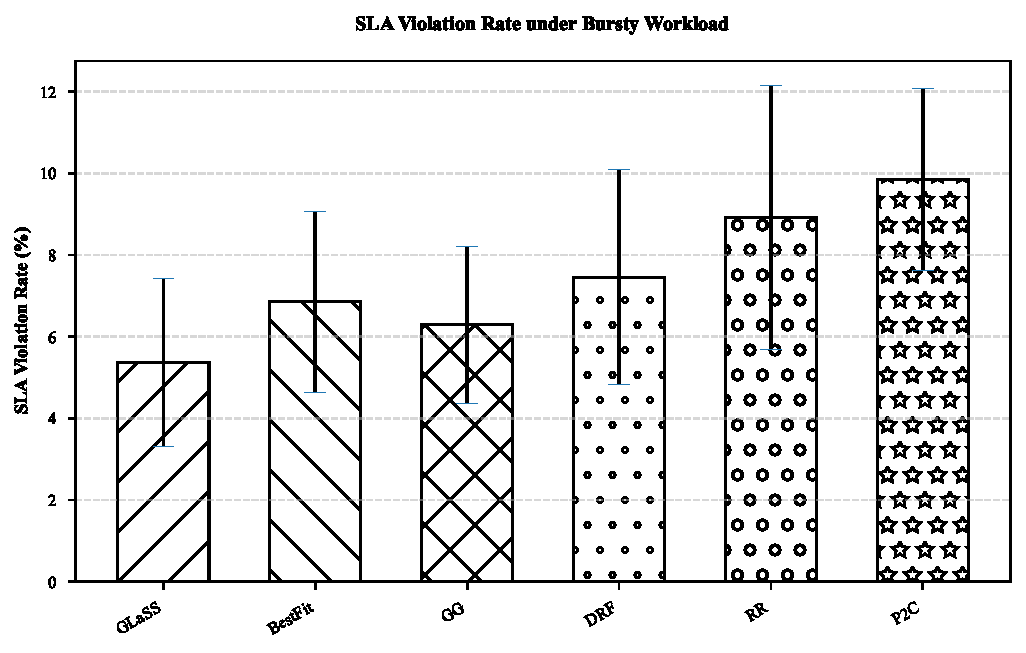
\includegraphics[width=0.95\linewidth]{SNN schedule/picture/sla_violation_comparison_bursty.pdf}
    \caption{SLA Violation Rate (Instantaneous load $> BW_{max}$) under Bursty Workloads. Baselines fail due to the lack of temporal interleaving.}
    \label{fig:sla}
\end{figure}

In event-driven neuromorphic computing, achieving spatial balance (Step A + C) is necessary but insufficient. SNN bursts occur in the microsecond domain. We measure temporal unbalance using the \textbf{SLA Violation Rate} (the percentage of clock cycles where a link's instantaneous injection rate exceeds $BW_{max}$).

\textbf{Counter-intuitive Insight: The Illusion of Average Bandwidth.} 
As shown in Fig.~\ref{fig:sla}, STPS achieves a remarkably low SLA violation rate of 5.37\%, thoroughly outperforming DRF (7.46\%) and BestFit (6.86\%). Because the baselines lack Step B, they inject task data immediately upon dispatch. Even if DRF perfectly balances the \textit{spatial average} load across cards, it is completely blind to temporal variance. Consequently, the biological "spike tides" of collocated bursty tasks randomly overlap, shattering the instantaneous $BW_{max}$ limit.

STPS introduces proactive \textbf{Temporal Flattening} through Step B. By leveraging the 1D traffic timeline fingerprint $E_{new}^{(t)}$, Step B executes a sliding-window cross-correlation to calculate an optimal clock offset $\Delta t_{start}^*$. This phase-shifting intentionally delays the task's execution onset by a few microseconds, forcing its burst peaks to fall perfectly into the temporal "valleys" of the background traffic. This zero-overhead temporal manipulation functionally acts as a traffic multiplexer, achieving mathematical temporal load balancing without adding any physical NoC bandwidth.

\subsection{Q3: Scalability and Ablation Study}
\label{sec:eval_scaling}

\begin{figure}[t]
    \centering
    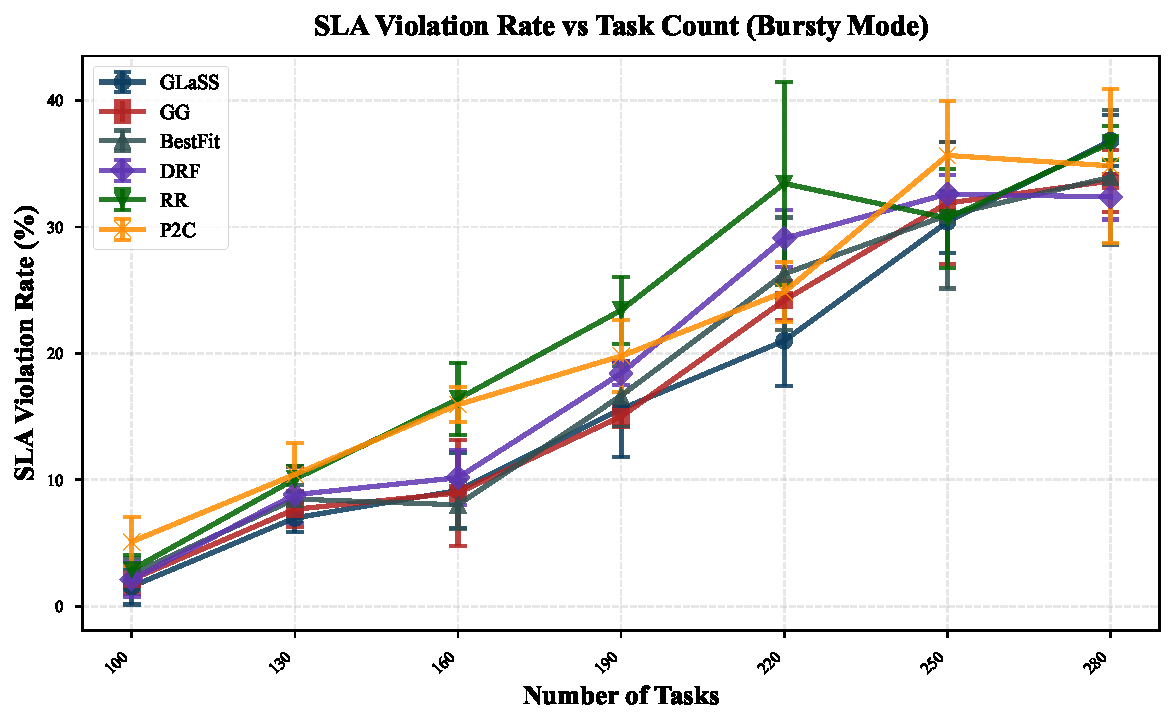
\includegraphics[width=0.95\linewidth]{SNN schedule/picture/task_scaling_sla.pdf}
    \caption{Impact of Task Density on SLA Violations. STPS unlocks hidden cluster capacity by treating time as an allocatable resource.}
    \label{fig:task_sla}
\end{figure}

To test the system limits and perform an ablation analysis, we scale the concurrent task count from 80 to 200 (Fig.~\ref{fig:task_sla}). 

\textbf{1) Unlocking Hidden Capacity (The critical role of Step B):} 
In the critical operating range (140--170 tasks), STPS demonstrates maximum superiority. At 160 tasks, STPS maintains a 21.0\% violation rate, outperforming BestFit (26.3\%) by 20.1\%. In this zone, physical spatial resources (Cores/Mem) are heavily fragmented. While static baselines trigger massive congestion, STPS safely "squeezes" newly arrived tasks into the remaining \textit{temporal voids} via Step B, delaying cluster saturation significantly longer than purely spatial schedulers. 

\textbf{2) Convergence at Physical Limits:} 
As tasks exceed 180 (utilization $\to$ 95\%), the SLA violation gaps among all schedulers narrow, with STPS converging to ~36.8\% at 200 tasks. This validates our analytical model: at extreme physical saturation, the background temporal traffic becomes a densely packed, flat high-water mark. The temporal variance approaches zero, leaving Step B with no valleys to exploit ($\Delta t_{start}^* \to 0$). At this limit, temporal load balancing naturally degrades, and STPS elegantly falls back to relying purely on its optimized spatial placement (Step A + C), proving its robustness across the entire load spectrum.

\section{Conclusion}
This paper presents GLaSS, a dynamic scheduler for SNN cloud services. By leveraging accumulated spike activity and ROI-based migration, GLaSS solves the static binding inefficiency inherent in neuromorphic hardware. Future work includes implementing predictive scaling based on historical spike patterns.


%-------------------------------------------------------------------------------
\section*{Acknowledgments}
%-------------------------------------------------------------------------------

The USENIX latex style is old and very tired, which is why
there's no \textbackslash{}acks command for you to use when
acknowledging. Sorry.

%-------------------------------------------------------------------------------
\section*{Availability}
%-------------------------------------------------------------------------------

USENIX program committees give extra points to submissions that are
backed by artifacts that are publicly available. If you made your code
or data available, it's worth mentioning this fact in a dedicated
section.

%-------------------------------------------------------------------------------
\bibliographystyle{plain}
\bibliography{references}

%%%%%%%%%%%%%%%%%%%%%%%%%%%%%%%%%%%%%%%%%%%%%%%%%%%%%%%%%%%%%%%%%%%%%%%%%%%%%%%%
\end{document}
%%%%%%%%%%%%%%%%%%%%%%%%%%%%%%%%%%%%%%%%%%%%%%%%%%%%%%%%%%%%%%%%%%%%%%%%%%%%%%%%

%%  LocalWords:  endnotes includegraphics fread ptr nobj noindent
%%  LocalWords:  pdflatex acks